% ==============================================================================
% SECTION 1: REGLEMENTATION
% ==============================================================================

\section{Réglementation \& Prérogatives}

\begin{frame}{Introduction}
    Les nouvelles prérogatives du N3 impliquent plus de responsabilités :
    \begin{itemize}
        \item Organiser une plongée et en assurer la sécurité en l'absence de Directeur de Plongée (DP).
        \item Respecter le cadre réglementaire (Code du Sport).
    \end{itemize}
\end{frame}

\begin{frame}{Objectifs}
    \textbf{À l'issue de ce cours, vous devrez :}
    \begin{itemize}
        \item Connaître vos prérogatives.
        \item Connaître vos contraintes matérielles.
        \item Connaître le cadre fédéral et les responsabilités.
        \item Maîtriser l'armement spécifique d'un bateau.
        \item Utiliser les procédures de sécurité.
        \item Savoir les perspectives d'évolution à partir du N3.
    \end{itemize}
\end{frame}

\begin{frame}{Les Prérogatives (Code du Sport)}
    \centering
    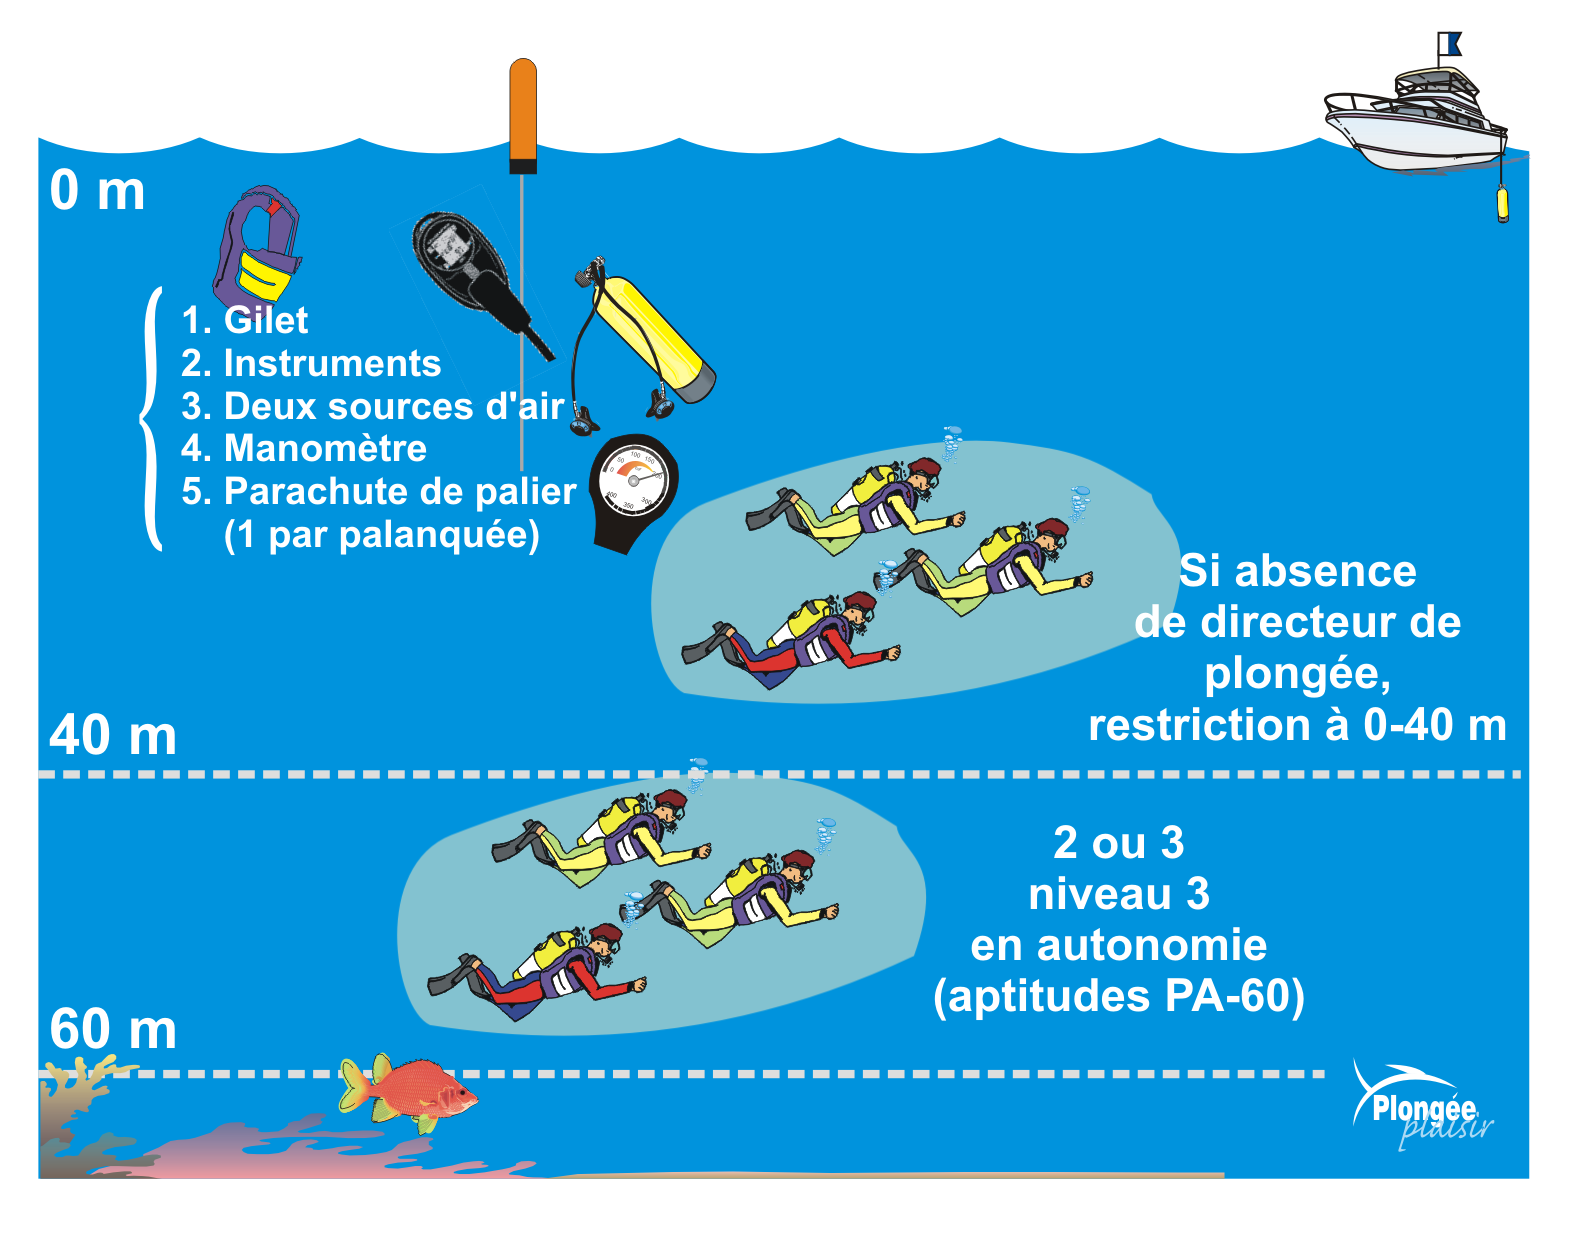
\includegraphics[height=0.9\textheight]{images/prerogative_n3}
\end{frame}

\begin{frame}{Les Prérogatives (Code du Sport)}
    \begin{block}{Le plongeur N3 FFESSM est :}
        \begin{itemize}
            \item \textbf{PA60} : Plongeur Autonome à 60m (si un DP est présent).
            \item \textbf{PA40} : Plongeur Autonome à 40m (en l'absence de DP).
            \item Équivalence CMAS 3*.
        \end{itemize}
    \end{block}

    \begin{alertblock}{Attention}
        \begin{itemize}
            \item Aucune équivalence directe avec PADI/SSI.
            \item Le RIFAP est un pré-requis obligatoire.
        \end{itemize}
    \end{alertblock}
\end{frame}

\begin{frame}{Matériel et Documents}
    \textbf{Matériel obligatoire (idem N2 + autonomie) :}
    \begin{itemize}
        \item Gilet.
        \item Instruments de décompression (ordinateur ou profondimètre + tables MN90).
        \item 2 sources d'air.
        \item Manomètre.
        \item Parachute de palier (1 par palanquée).
    \end{itemize}

    \vspace{0.5cm}
    \textbf{Documents nécessaires :}
    \begin{itemize}
        \item \textbf{Licence} : Assurance RC, valide du 01/09 au 31/12 (année suivante).
        \item \textbf{CACI} (Certificat Médical d'absence de contre-indication) : Moins d'un an dans les clubs associatifs.
        \item \textbf{Carnet de plongée} : Justifie l'expérience auprès des centres.
    \end{itemize}
\end{frame}

\begin{frame}{Responsabilité}
    \begin{block}{Responsabilité du Plongeur Autonome N3}
        En l'absence de DP, le plongeur N3 est responsable de :
        \begin{itemize}
            \item La planification de la plongée (site, profondeur, durée, DTR).
            \item La sécurité de la palanquée (matériel, procédures, secours).
            \item Le respect de la réglementation (prérogatives, matériel).
        \end{itemize}
    \end{block}

    \begin{alertblock}{Attention}
        Une mauvaise gestion peut engager votre responsabilité civile et \textbf{pénale} en cas d'accident.
    \end{alertblock}
\end{frame}

\begin{frame}{Responsabilités et Assurances}
    \centering
    
    \begin{tikzpicture}[
        scale=0.85, transform shape,
        % Styles globaux (Notez l'absence de lignes vides ici)
        base/.style={align=center, font=\small},
        % Style "Cause" (Haut)
        box_cause/.style={base, fill=FillCause, text=PrimaryColor, text width=3cm, minimum height=1.2cm, inner sep=5pt},
        % Style "Concept" (Milieu)
        box_concept/.style={base, fill=FillConcept, text=white, text width=3.2cm, minimum height=1.2cm, font=\bfseries\small},
        % Style "Description" (Bas)
        text_desc/.style={base, text=PrimaryColor, text width=3.5cm, node distance=1.5cm},
        % Style des flèches
        arrow/.style={->, >={Latex[length=3mm]}, thick, PrimaryColor},
        % Espacement global
        node distance=0.8cm and 0.3cm
    ]

    % --- COLONNE 1 (GAUCHE) ---
    \node[box_cause] (top1) {Infraction\\à la loi};
    \node[box_concept, below=of top1] (mid1) {Responsabilité\\pénale};
    \node[text_desc, below=of mid1] (bot1) {Pas d'assurance\\mais un contrat RC\\peut prévoir une\\protection juridique};

    % --- COLONNE 2 (CENTRE) ---
    \node[box_cause, right=of top1] (top2) {Préjudice causé\\à un tiers};
    \node[box_concept, below=of top2] (mid2) {Responsabilité\\civile};
    \node[text_desc, below=of mid2] (bot2) {Assurance en RC\\(dommages et\\intérêts)\\\textcolor{AlertColor}{\textbf{Obligatoire}}};

    % --- COLONNE 3 (DROITE) ---
    \node[box_cause, right=of top2, text width=3.5cm] (top3) {Dommages\\\textbf{corporels} sans\\tiers responsable};
    
    % Note : le "-|" permet d'aligner verticalement sous mid2 mais horizontalement avec top3
    \node[text_desc, below=of mid2 -| top3] (bot3) {Assurance individuelle\\Assistance, rapatriement\\[1em]\textcolor{AlertColor}{Facultatif en loisir}};

    % --- FLÈCHES ---
    \draw[arrow] (top1) -- (mid1);
    \draw[arrow] (mid1) -- (bot1);
    \draw[arrow] (top2) -- (mid2);
    \draw[arrow] (mid2) -- (bot2);
    \draw[arrow] (top3) -- (bot3);

    % --- ARRIÈRE-PLAN ---
    \begin{scope}[on background layer]
        \node[fit=(top1)(bot3)(top3), fill=CanvasBg, draw=PrimaryColor!50, inner sep=15pt, rounded corners=0pt] {};
    \end{scope}

    \end{tikzpicture}
\end{frame}